\section{Conditionals}

\subsection{If Else Statements}
\begin{frame}[fragile]{If and Else}{}
    \begin{block}{}
        The \textbf{else} statement is optional.
    \end{block}
    \begin{minted}{c++}
        if (temperature >= 38)
            cout << "Buy an ice ceam cone" << endl;
        else
            cout << "Buy a lollipop" << endl;
    \end{minted}
    \begin{block}{}
        Must use a block (surrounded by curly braces) for more than one line.
    \end{block}
    \begin{minted}{c++}
        if (number_of_lines > 1) {
            cout << "More than one line.";
            cout << "Have to use a block.";
        }
        else{
            cout << "Curly braces are optional.";
        }
    \end{minted}
\end{frame}

\begin{frame}[fragile]{The \textbf{if...else if...else} Statement}{}
    \begin{center}
        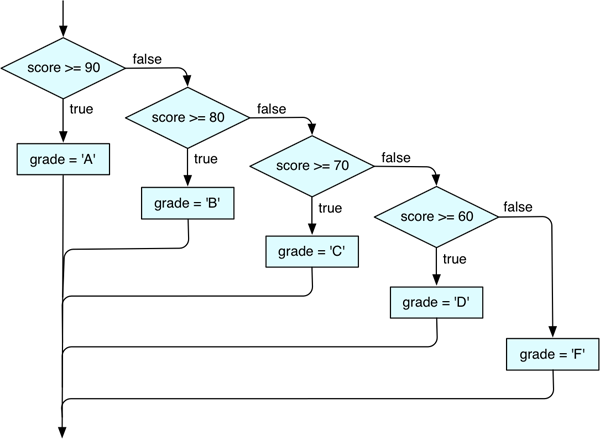
\includegraphics[width=.8\linewidth]{images/elseif.png}
    \end{center}
\end{frame}

\begin{frame}[fragile]{The \textbf{if...else if...else} Statement}{}
    \begin{block}{}
        To test multiple conditions, we can cascade if statements
    \end{block}
    \begin{minted}{c++}
        if (temperature >= 35) {
            cout << "Buy an ice ceam cone" << endl;
        }
        else if (temperature >= 25) {
            cout << "Buy a lollipop" << endl;
        }
        else if (temperature >= 15) {
            cout << "Buy a coffee" << endl;
        }
        else {
            cout << "Buy a sweater !" << endl;
        }
    \end{minted}
\end{frame}

\begin{frame}[fragile]{The \textbf{if...else if...else} Statement}{}
    \begin{itemize}
        \item The first statement must be an \emph{if}.
        \item After this, there can be any number of \emph{if else} statements. 
        \item At the end, there can be one (or zero) \emph{else} statement. 
    \end{itemize}
\end{frame}

\subsection{Nested Conditionals}
\begin{frame}[fragile]{Nested Conditionals}{}
    \begin{center}
        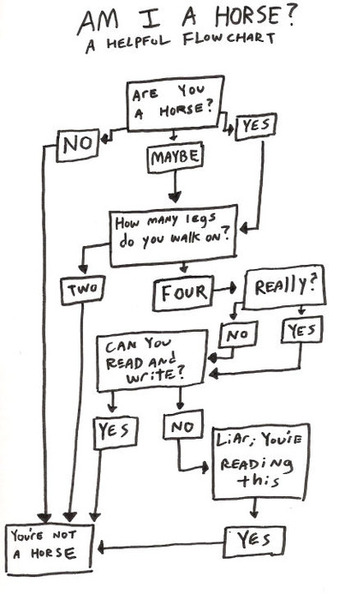
\includegraphics[width=.4\linewidth]{images/horse.jpg}
    \end{center}
\end{frame}

\begin{frame}[fragile]{Nested Conditionals}{}
    \begin{minted}{c++}
        if (temperature >= 35) {
            if (money >= 45) {
                cout << "Buy a Cornetto" << endl;
                money -= 45;
                if (money > 0) {
                    cout << "Buy a candy" << endl;
                }
                else
                    cout << "Out of Money :(" << endl;
            }
            else
                cout << "Buy a Pepsi" << endl;
        }
        else {
            cout << "Buy a lollipop" << endl;
        }
    \end{minted}
\end{frame}
